\documentclass[a4paper,12pt]{scrartcl}

\usepackage[utf8]{inputenc}
\usepackage[french]{babel}
\usepackage{graphicx}
\usepackage{subcaption}

\title{Projet électronique - Rapport intermédiaire}
\subject{\texttt{2T2072} - Groupe 04}
\author{
  Julien Claerhout
  \and Maxence Demaiffe
  \and Morgane Leclerc
  \and Habibou Moulaye Zeini
  \and Jérôme Verkyndt
}

\begin{document}

\maketitle

\section{Objectifs du projet}

Il nous est demandé de réaliser une carte avec un télémètre à ultrasons qui
enverra à un microcontrôleur (Raspberry Pi PICO) la mesure de la distance qui
le sépare de l’entité se trouvant devant lui. La distance sera affichée sur 2
afficheurs 7 segments et la carte devra afficher en permanence une LED verte
lorsqu’il n’y a pas d’alerte et une LED clignotante rouge lorsque la distance
tombe en dessous d’un seuil critique défini par l’utilisateur. Pour finir, le
Raspberry Pi PICO devra être capable de communiquer avec une application python
qui affichera la distance et qui nous permettra de changer le seuil d’alerte.

\section{R\'epartition du travail au sein du groupe}

Tous les étudiants du groupe se sont d’abord familiarisé avec le logiciel
Eagle (explications en cours, tutoriels) avant de commencer à travailler sur le
projet. Une fois le logiciel pris en main, nous avons travaillé en équipe sur
la conception du schéma.

\section{
  Sch\'ema \'electronique finalis\'e et d\'efinitif de la carte dans Eagle
}

Le Raspberry pi pico contrôle 4 shift-registers 4-bits (\textsc{74LS194}) en
série. La pin de contrôle de mode \texttt{S1} est maintenue à $0$, tandis que
\texttt{S0} est branchée à une GPIO du pico. Lorsque celle-ci est à $0$, les
registres sont en mode \textit{hold} et maintiennent leurs valeurs. Si elle
est à $1$, le premier registre de la chaîne va alors échantillonner la valeur
à la pin \texttt{DSR} (contrôlée par le pico) de la première puce et décaler
les autres, permettant ainsi de convertir un signal en série du pico. La pin
\texttt{Q3} de chaque registre est branchée à la pin \texttt{DSR} du suivant,
créant ainsi une chaîne de 16-bits. La pin \texttt{Q3} du dernier registre est
simplement branchée à son segment d'afficheur.

Contrôller les afficheurs est alors un processus en 5 étapes simples:
\begin{enumerate}
  \item On éteint les afficheurs en coupant le courant de base des transistors
    branchés aux cathodes des afficheurs.
  \item On active les pins \texttt{S1}
    de tout les registres. Ils ne sont désormais plus bloqués et vont pouvoir
    accepter des données du pico.
  \item Pour chaque segment des afficheurs,
    on met la pin \texttt{DSR} du premier registre \textit{low} (pour qu'il
    soit éteint) ou \textit{high} (pour l'allumer), puis on déclenche un
    \textit{rising edge} sur les pins \texttt{CP} des registres. Chaque bit
    enregistré sera alors décalé à droite.
  \item On désactive les pins \texttt{S1} des registres, bloquant les valeurs
    enregistrées et empêchant plus de données d'être acceptées.
  \item On allume les afficheurs en activant un courant à la base des
    transistors branchés aux cathodes des afficheurs.
\end{enumerate}

\begin{figure}
  \centering
  % TODO: Replicate it in tikz lmao
  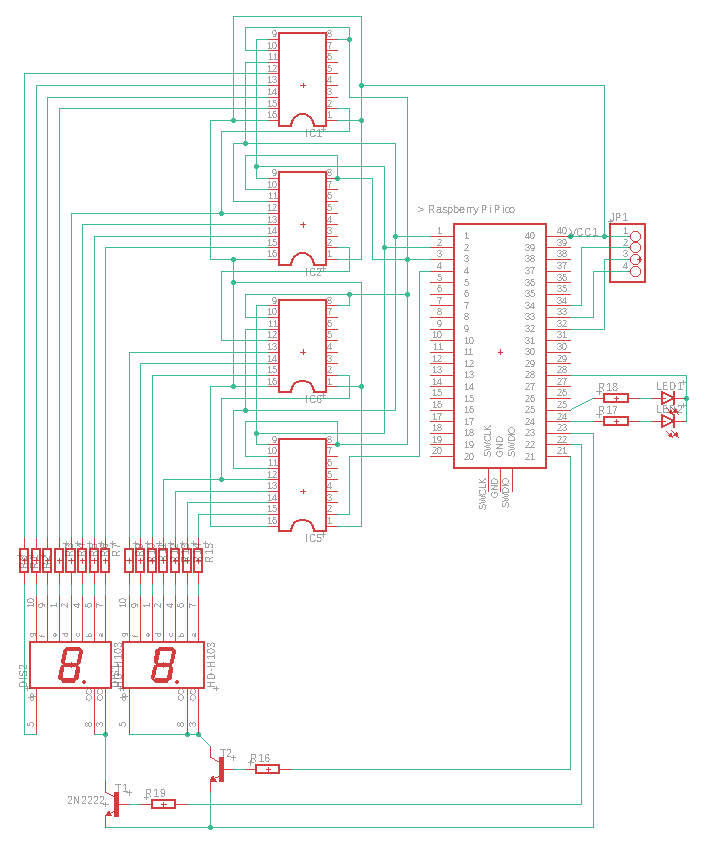
\includegraphics[width=0.5\textwidth]{sonic-telemeter-schematic.png}
  \caption{\label{fig:schematic}: Schéma du télémètre}
\end{figure}

\begin{figure}
  \centering
  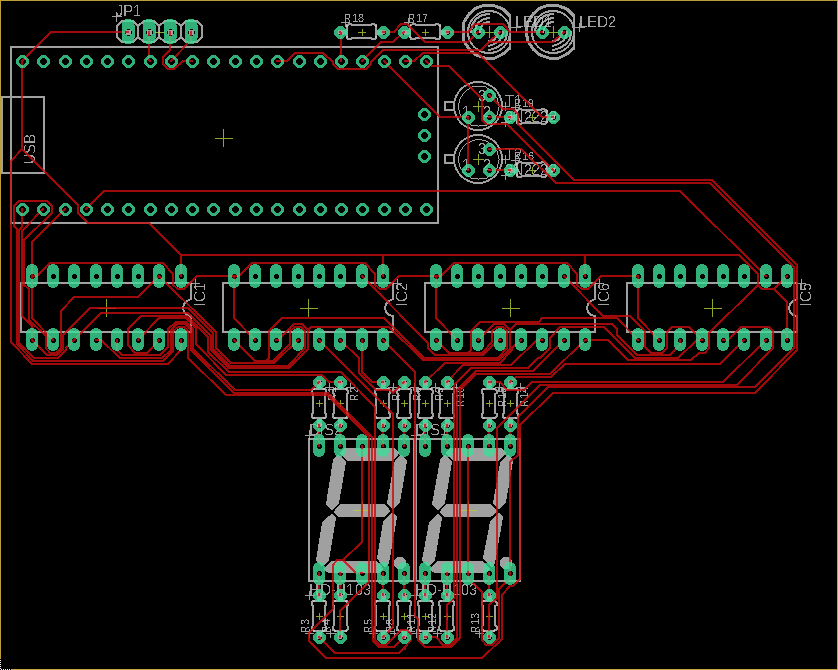
\includegraphics[width=0.7\textwidth]{sonic-telemeter-board.png}
  \caption{\label{fig:board}: Design de la carte du télémètre}
\end{figure}

\begin{table}
  \centering
  \begin{tabular}{c|c|l|r}
    \textbf{pin n°} & \textbf{nom} & \textbf{fonction} & \textbf{branchement}
    \cr
    \texttt{1} & \texttt{DDW} & Display data write & Pin \texttt{S1} de chaque
      shift-register
    \cr
    \texttt{2} & \texttt{DCK} & Display data clock & Pin \texttt{CP} de chaque
      shift-register
    \cr
    \texttt{4} & \texttt{DDS} & Display data serial & Pin \texttt{DSR} du
      premier shift-register
    \cr
    \texttt{21},\texttt{22} & \texttt{DEN} & Display enable & Bases des
      transistors
    \cr
    \texttt{24},\texttt{25} & \texttt{AL1}, \texttt{AL2} & Alert led 1 \& 2 &
      Anode des leds
    \cr
    \texttt{32} & \texttt{SECH} & Sensor echo & Pin \texttt{ECHO} de la sonde
      ultrasons.
    \cr
    \texttt{34} & \texttt{STRG} & Sensor trigger & Pin \texttt{TRIG} de la
      sonde ultrasons.
    \cr
    \texttt{3},\texttt{23},\texttt{28},\texttt{33} & \texttt{GND} & terre &
      \texttt{S0} de chaque shift-register
    \cr
    \texttt{40} & \texttt{VCC} & alimentation $5V$ & \texttt{MR} de chaque
      shift-register
  \end{tabular}
  \caption{\label{tab:pinout} Utilisation des pins du pi pico}
\end{table}

\section{État d'avancement de la programmation}

Une simulation fonctionnelle permettant de gérer l’affichage sur 7-segments  a
été réalisée sur Wokwi. Toutefois, il convient de noter que cette simulation
s’est faite avec les composants disponibles sur le site. Ces composants
ne sont pas toujours les mêmes dont nous disposons en laboratoire. La plus
grande différence est que sur Wokwi on utilise des registres à décalages
74HC595 tandis qu’au laboratoire ce sont des 74LS194 4-bits. La simulation
met une alternance de 1 et de 0 des registres à décalages et les envoie sur un
afficheur 7 segments.

\section{État d'avancement général}

Au vu de ce qui précède, il ressort que le projet est en bonne voie. Au niveau
du hardware le schematic vient d'être finalisé. Une fois le circuit reçu, il
ne restera plus qu’à tester son bon fonctionnement et y raccorder les autres
éléments.  En ce qui concerne la programmation, nous comptons continuer sur la
base que nous avons déjà afin de peaufiner la gestion de l’affichage à la fois
sur les afficheurs et sur le programme python. Avant cela, la communication
devrait être établie entre le microcontrôleur et le programme python.

\end{document}
